% Section content template for individual Educative lessons
% This file contains the actual content for a specific section
% Generated from Educative API section content

% Section: Use Case Diagram
% Section ID: 5424575903170560
% Section Slug: use-case-diagram
% Generated: 2025-12-08T22:21:20.076546

\textbf{Use case diagram} describes the specification of users and their possible interactions with the system. These possible interactions are called \textbf{use cases.}

\subsection{Components of a use case diagram}\label{Jr3OajG2dAjHnSXH9Sd1A}
\\
To understand a use case diagram, it is important to first understand its components. Use case diagrams have the following components:

\begin{itemize}
\item
\protect\phantomsection\label{efg0yvEHWCt7TJnPVBV-I}
\textbf{Actor:} Users are called actors. They interact with the system. They could be humans, machines/hardware, or other external systems. There are two types of actors:

\begin{itemize}
\item
\textbf{Primary actors:} These are the humans or external systems that interact with that system and are responsible for initiating the use case. They are placed on the left side in a use case diagram. Primary actors are also called \textbf{active actors}.
\item
\textbf{Secondary actors:} These are the ones that are used by the system to assist the primary actors in a use case. They cannot interact with the system on their own. They need primary actors to initiate a use case. Secondary actors are also called \textbf{passive actors}, and they are placed on the right side in a use case diagram.
\end{itemize}
\item
\protect\phantomsection\label{L0nZh3f8sQFOoBiqVjLrj}
\textbf{Use case:} This is a single function performed on a system by an actor. It is represented by an oval shape.
\item
\protect\phantomsection\label{MjTQrixB2OhNn298U25Ln}
\textbf{Package:} This is a group of different elements. These groups are represented inside a folder icon.
\item
\protect\phantomsection\label{e0T4q0daArvBA4Jg7GcO8}
\textbf{Note:} This is used to add additional information about any component or relationship in a use case diagram.
\end{itemize}
\\
The representation of the components explained above in a use case diagram is given below:

\begin{figure}[htbp]
 \centering
 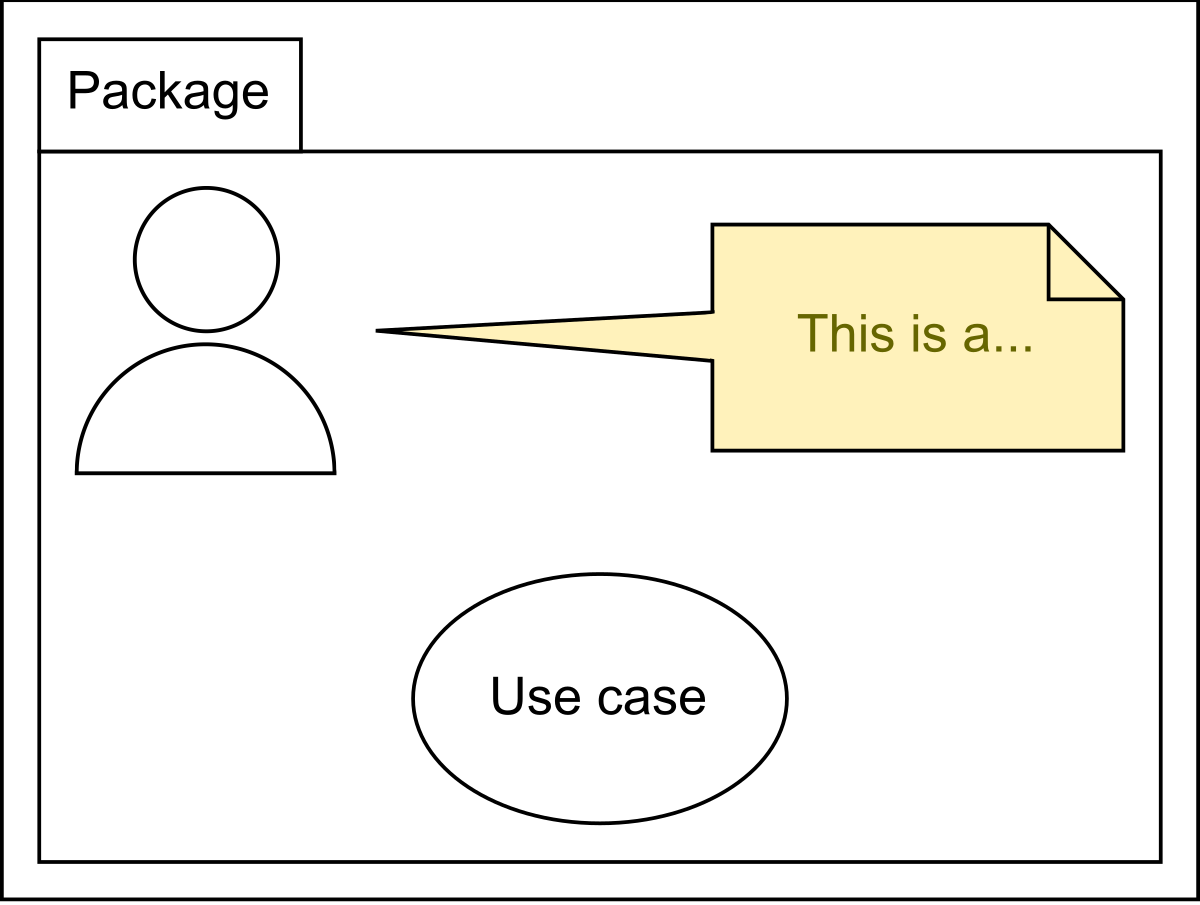
\includegraphics[width=0.25\textwidth]{Images/chapter_3/section_5424575903170560/4814649419890688.png}
 \caption{Components of a use case diagram}
\end{figure}

\subsection{Relationships in use case diagrams}\label{7LmzMXzNyuk8mZ9yC1ZlD-2}
\\
There are four different types of relationships in a use case diagram:

\begin{enumerate}
\item
\protect\phantomsection\label{sH4VAlyTZUgGBEw2DLNDZ}
\textbf{Association:} This shows the relationship between and among actor(s) and use case(s). It represents how an actor can perform certain functions. It is denoted by a solid line without arrows. All the actors in a use case diagram must have at least one association with any use case. More than one actor can be associated with the same use case, and a single actor can be associated with more than one use case.
\item
\protect\phantomsection\label{f0Ieq0Lf8AQKe0N0oNghW}
\textbf{Generalization:} This relationship is also known as inheritance. In inheritance, we have parent and children classes. Similarly, in a use case diagram, we have parent and child use cases. The child use case has generalization with the parent use case. Each child inherits the behavior of its parent. It is denoted by a solid line with an arrow on only one side (toward the parent use case).
\item
\protect\phantomsection\label{6BvPQywxfFuc_rtqOG0A6}
\textbf{Include:} We use this to show the relationship between two use cases. It shows that one use case includes the behavior of another use case. The included use case will execute only after the execution of the base use case. We can also say that the base use case requires an included use case in order to be completed. It is represented by a dashed line with an arrow on only one side (toward the included use case), and we write \textless{\textless{} include\textgreater{}\textgreater{}} above the line.
\item
\protect\phantomsection\label{_I1q_yrurL7cOy8UhK9AL}
\textbf{Extend:} We use this to show the relationship between two use cases. It shows that one use case extends the behaviors of another use case. The extended use case does not execute every time. It always depends on certain conditions. It is used to extend the functionality of the base use case. It is represented by a dashed line with an arrow on only one side (toward the base use case), and we write \textless{\textless{} extend\textgreater{}\textgreater{}} above the line.
\end{enumerate}
\\
In the example below, we have a small ATM (automated teller machine) transaction system where customers can transfer funds and make payments. To validate the funds, the transfer system has to check if a sufficient amount of funds is available. Otherwise , an error message will be displayed. To make a payment, a customer has two choices. It can either pay via a current account or a savings account.

\begin{figure}[htbp]
 \centering
 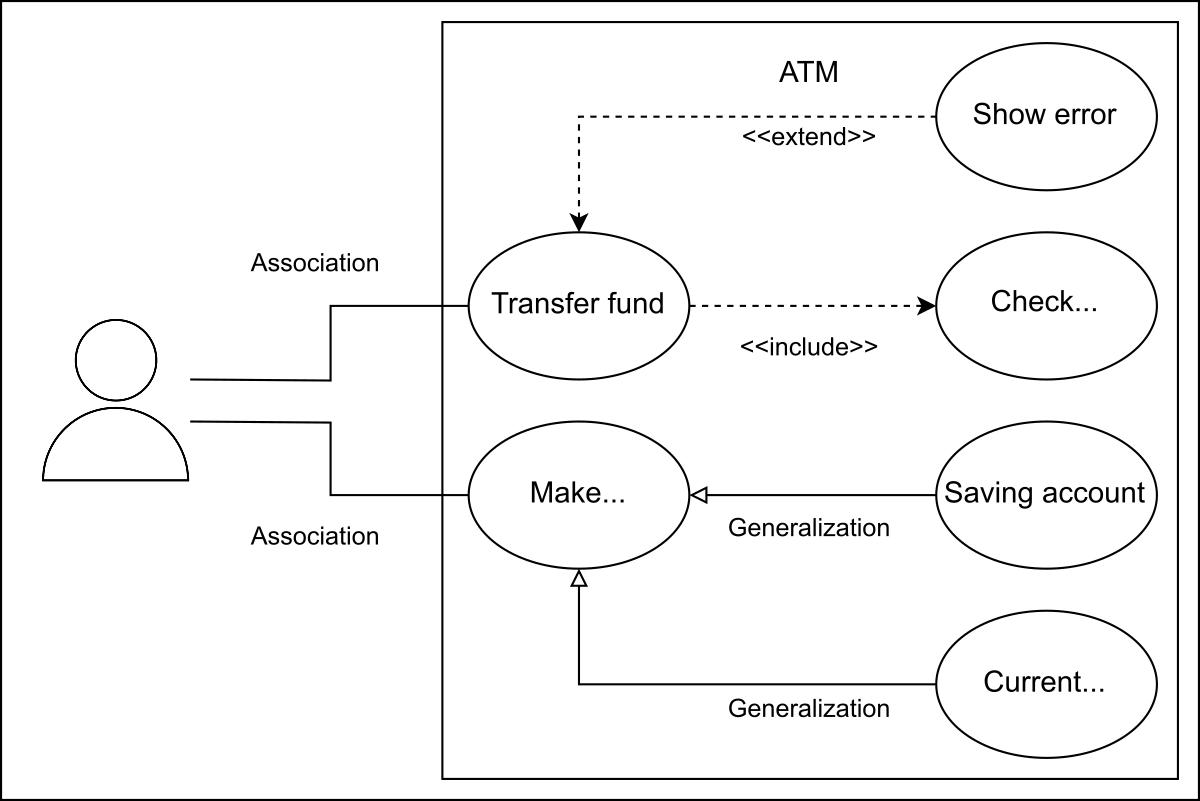
\includegraphics[width=0.5\textwidth]{Images/chapter_3/section_5424575903170560/6119153444061184.png}
 \caption{The use case diagram of an ATM}
\end{figure}

\subsection{Benefits of use case diagrams}\label{yi1KJ4RUiyJ7Uwoj5VcrT}
\\
A use case diagram is important in the following scenarios:

\begin{itemize}
\item
\protect\phantomsection\label{4-cnFgF8oLTWuNiDHAyzN}
It explains the flow and objective of all use cases.
\item
\protect\phantomsection\label{VcT8hBtITtHRjmvKPRTw0}
It helps in understanding the high-level functional requirements of the system.
\item
\protect\phantomsection\label{xsu7u5GBGzGLv7EJ3Ttux}
It defines a system\textquotesingle s context and needs.
\item
\protect\phantomsection\label{zM98PT4JTnZhMyublJE8x}
It explains system behavior from a user perspective.
\item
\protect\phantomsection\label{rW4Ml4_181jIOirw6nijS}
It explains the scope of the system.
\end{itemize}
\\
In the next lesson, we will discuss the class diagram with its components in detail.

% End of section content